\section{截交线与相贯线}
\subsection{截交线}
 机器零件通常需要加工一些斜切口或开槽,这些结构可以看作是一个或多个平面切割立体而成。这些平面或曲面截切立体所产生的表面交线称之为截交线。
 \subsubsection{平面与棱柱的交线}
图\ref{fig:jiejiao1}为倾斜于正六棱柱轴线且过顶面的截面切割的结果,其截面为五边形封闭线框。由图\ref{fig:jiejiao2}所示的三视图可知,该封闭线框构成的平面区域垂直于$V$投影面,投影为一积聚直线,其俯视图和左视图投影为类似形的封闭五边形,结果如。
 \begin{figure}[htbp]
 \centering
\subfloat[]{\label{fig:jiejiao1}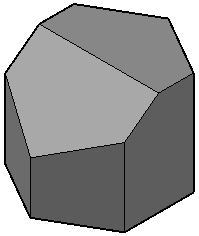
\includegraphics[scale=0.8]{jiejiao1.png}}\hspace{30pt}
\subfloat[]{\label{fig:jiejiao2}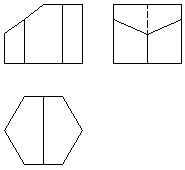
\includegraphics[scale=1]{jiejiao2.png}}
\caption{正六棱柱的截交线}
\end{figure}
\subsubsection{平面与棱锥的交线}
 \begin{figure}[htbp]
 \centering
\subfloat[]{\label{fig:jiejiao3}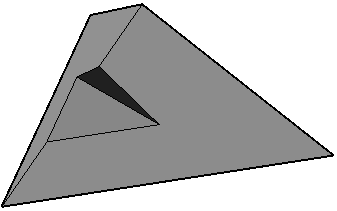
\includegraphics[scale=0.6]{jiejiao3.png}}\hspace{30pt}
\subfloat[]{\label{fig:jiejiao4}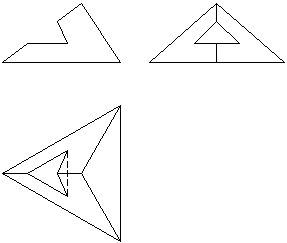
\includegraphics[scale=0.65]{jiejiao4.png}}
\caption{正三棱锥的截交线}
\end{figure}
图\ref{fig:jiejiao3}为两个截平面切割正三棱锥的结果,其截面由两个三角形封闭线框构成。从图\ref{fig:jiejiao4}所示的三视图可知,其中一个截平面平行于$H$面,另一个截平面垂直于$V$面,水平截的投影在主视图和左视图中积聚为水平直线,正垂截面的俯视图投影和左视图投影为类似形的三角形封闭线框。

\subsubsection{平面与圆柱体的交线}
 \begin{figure}[htbp]
 \centering
\subfloat[]{\label{fig:jiejiao5}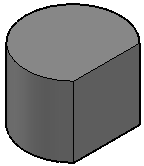
\includegraphics[scale=0.7]{jiejiao5.png}}\hspace{60pt}
\subfloat[]{\label{fig:jiejiao6}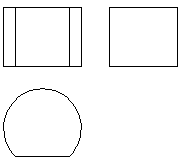
\includegraphics[scale=0.8]{jiejiao6.png}}
\caption{截交面与轴线平行}
\end{figure}
图\ref{fig:jiejiao5}为平行于轴线的截交平面切割圆柱体后的结果,其截面是由一矩形构成封闭线框。从图\ref{fig:jiejiao6}所示的三视图可知,截平面平行于$V$面,其主视图投影为一反映实形的矩形,其余视图投影为一积聚的直线。

\begin{figure}[htbp]
\centering
\subfloat[]{\label{fig:jiejiao7}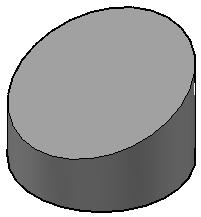
\includegraphics[scale=0.6]{jiejiao7.png}}\hspace{60pt}
\subfloat[]{\label{fig:jiejiao8}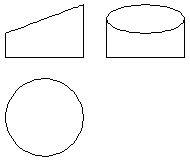
\includegraphics[scale=0.75]{jiejiao8.png}}
\caption{截交面倾斜于轴线且不交于上下表面}
\end{figure}
图\ref{fig:jiejiao7}为倾斜于轴线且不与上下表面相交的截交面切割圆柱体后的结果,其截面为椭圆曲线构成的封闭线框。由图\ref{fig:jiejiao8}所示的三视图可知,该封闭线框构成的平面垂直于$V$面,其主视图投影积聚为一条直线,俯视图投影为一正圆,左视图投影为。

\begin{figure}[htbp]
\subfloat[]{\label{fig:jiejiao9}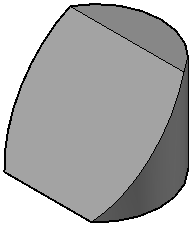
\includegraphics[scale=0.6]{jiejiao9.png}}\hspace{60pt}
\subfloat[]{\label{fig:jiejiao10}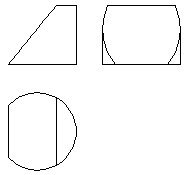
\includegraphics[scale=0.8]{jiejiao10.png}}
\caption{截交面倾斜于轴且交于上下表面}
\end{figure}
图\ref{fig:jiejiao9}为倾斜于轴线且与上下表面相交的截交面切割圆柱体的一结果,其截面是由直线和椭圆曲线共同构成的复合图形。由图\ref{fig:jiejiao10}所示的三视图可知,该封闭线框垂直于$V$面,其主视图投影积聚为一直线,其俯视图和左视图为类似形的复合图形。

\subsubsection{圆锥截交体}
 \begin{figure}[htbp]
 \centering
\subfloat[]{\label{fig:jiejiao11}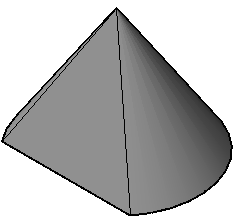
\includegraphics[scale=0.4]{jiejiao11.png}}\hspace{60pt}
\subfloat[]{\label{fig:jiejiao12}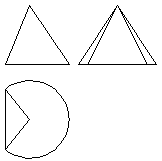
\includegraphics[scale=0.6]{jiejiao12.png}}
\caption{截交面过锥顶}
\end{figure}
图\ref{fig:jiejiao11}为截交面通圆锥体锥顶,其截交线为三角形,图\ref{fig:jiejiao12}为其三视图;

\begin{figure}[htbp]
\centering
\subfloat[]{\label{fig:jiejiao13}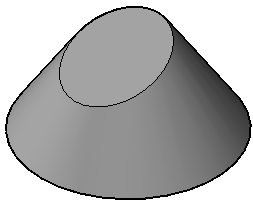
\includegraphics[scale=0.4]{jiejiao13.png}}\hspace{60pt}
\subfloat[]{\label{fig:jiejiao14}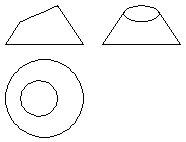
\includegraphics[scale=0.6]{jiejiao14.png}}
\caption{截面倾斜于轴线且倾斜角度大于锥角}
\end{figure}
图\ref{fig:jiejiao13}为截面倾斜于轴线且倾斜角度大于锥角,其截交线为椭圆,图\ref{fig:jiejiao14}为其三视图;

\begin{figure}[htbp]
\centering
\subfloat[]{\label{fig:jiejiao15}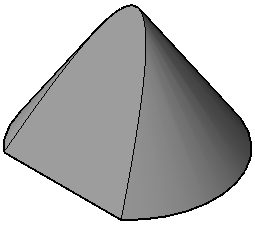
\includegraphics[scale=0.4]{jiejiao15.png}}\hspace{60pt}
\subfloat[]{\label{fig:jiejiao16}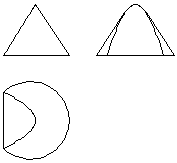
\includegraphics[scale=0.6]{jiejiao16.png}}
\caption{截面倾斜于轴线且倾斜角度等于锥角}
\end{figure}
图\ref{fig:jiejiao15}为截面倾斜于轴线且倾斜角度等于锥角,其截交线为抛物线,图\ref{fig:jiejiao16}为其三视图;

\begin{figure}[htbp]
\centering
\subfloat[]{\label{fig:jiejiao17}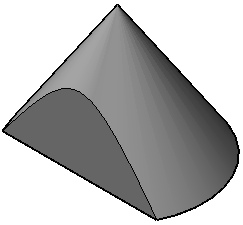
\includegraphics[scale=0.4]{jiejiao17.png}}\hspace{60pt}
\subfloat[]{\label{fig:jiejiao18}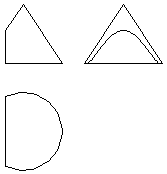
\includegraphics[scale=0.6]{jiejiao18.png}}
\caption{截面与轴线平行}
\end{figure}
图\ref{fig:jiejiao17}为截面与轴线平行,其截交线为双曲线,图\ref{fig:jiejiao18}为其三视图。
\endinput
 